\documentclass{article}
\usepackage[T1]{fontenc}
\usepackage{booktabs}
\usepackage{siunitx}
\usepackage{placeins}
\usepackage{lineno}
\usepackage{graphicx}
\newcolumntype{d}{S[input-symbols = ()]}

\renewcommand{\thefigure}{S-\arabic{figure}}
\renewcommand{\thetable}{S-\arabic{table}}
\renewcommand{\theequation}{S-\arabic{equation}}
\renewcommand{\thesection}{S}
\renewcommand{\thelinenumber}{S-\arabic{linenumber}}
\renewcommand{\thepage}{Supp.Mat. page \arabic{page}}

\begin{document}


\title{Strong spatial and temporal limitation in seed arrival as  complementary mechanisms for species coexistence in a tropical Atlantic coastal forest}


\author{Leticia B. Zimback, Paulo I. Prado, Marcelo P. Pansonato, \\ Geraldo A. D. C. Franco,  
Adriana M. Z. Martini}

\date{\Large Supplementary Information}

\maketitle

%\section{Model selection and average models}
%\label{sec:model-select-aver}

In this %section
appendix
we report the coefficients of the selected models
($\Delta \mathrm{AIC} \leq 2$) to describe spatial seed limitation
(\emph{SSL}, equation 1 in Methods in the main paper) and temporal
seed limitation (\emph{TSL}, equation 2). We also provide the AIC
values for each model and the coefficients for the average model,
obtained from the selected models.


The set of competing models have as linear predictors all combinations
of the following fixed effects and their interactions (see methods in
the main paper for details):

\begin{description}
\item[Log seed mass]: logarithm dry seed mass average of each plant species
\item[Adult maximum height]:  maximum tree height recorded in the study site \cite{pansonato2018}.
\item[Frequency of adults]: proportion of the sampling plots in which adults of each species was recorded \cite{pansonato2018}. 
\end{description}

All these fixed-effect variables were standardized as z-values, to
ease convergence fo the mixed-effect models, and also to allow
comparison of the coefficients for each effect. We thus refer the
coefficients as ``standardized coefficients'' in the tables below.

We evaluated two response variables to express SSL: (i) the proportion
of seed traps where seeds of each species were not recorded each year,
and (ii) the proportion of traps where seeds of each species were
never recorded in any of the three sampling years. Accordingly, TSL
was also assessed by two response variables: (i) proportion of
sampling occasions (months) when seeds of each species were not
recorded in some trap, and (ii) proportion of the twelve months of the
year when seeds of each species were not recorded over the three
sampling years. As all response variables are proportions, we used
generalized binomial models.

Response variables (i) have three values for each species, which
correspond to the proportions of unoccupied traps or unnocupied
occasions each sampling year. We thus included in the model for these
responses a random effect for plant species. Plots with the values of
these responses and values predicted by the models are in the main
text. For response variables (ii) we used linear models only with the fixed
effects, as there is no repeated responses for each plant species.
Figures~\ref{fig:SSL_glm}~and~\ref{fig:TSL_glm} show the values of the responses
(ii) and the values predicted by the models. 

\FloatBarrier

\begin{table}

\caption{Mixed-effect models for the spatial seed limation. For each model is shown standarzide coefficients and standard error (brackets).}
\centering
\begin{tabular}[t]{lccccccc}
\toprule
  & 8 & 16 & 7 & 24 & 32 & 6 & Average\\
\midrule
Adult Frequency & \num{-0.410} & \num{-0.303} &  & \num{-0.445} & \num{-0.334} & \num{-0.618} & \num{-0.407}\\
 & (\num{0.226}) & (\num{0.231}) &  & (\num{0.224}) & (\num{0.227}) & (\num{0.218}) & (\num{0.249})\\
Adult height & \num{-0.478} & \num{-0.542} & \num{-0.659} & \num{-0.467} & \num{-0.536} &  & \num{-0.531}\\
 & (\num{0.231}) & (\num{0.227}) & (\num{0.217}) & (\num{0.226}) & (\num{0.221}) &  & (\num{0.238})\\
Log seed mass & \num{1.018} & \num{1.024} & \num{0.975} & \num{1.003} & \num{1.009} & \num{1.029} & \num{1.010}\\
 & (\num{0.205}) & (\num{0.197}) & (\num{0.214}) & (\num{0.201}) & (\num{0.192}) & (\num{0.220}) & (\num{0.208})\\
Frequency:Height &  & \num{-0.320} &  &  & \num{-0.335} &  & \num{-0.326}\\
 &  & (\num{0.234}) &  &  & (\num{0.228}) &  & (\num{0.235})\\
Frequency:Mass &  &  &  & \num{0.257} & \num{0.268} &  & \num{0.262}\\
 &  &  &  & (\num{0.224}) & (\num{0.214}) &  & (\num{0.223})\\
SD (Intercept) & \num{1.022} & \num{0.979} & \num{1.085} & \num{1.002} & \num{0.952} & \num{1.113} & \\
SD (Observations) & \num{1.000} & \num{1.000} & \num{1.000} & \num{1.000} & \num{1.000} & \num{1.000} & \\
\midrule
AIC & \num{489.1} & \num{489.3} & \num{490.2} & \num{489.8} & \num{489.8} & \num{491.0} & \\
\bottomrule
\end{tabular}
\end{table}


\begin{table}
\label{tab:SSL_glm}
\caption{Mixed-effect models for the temporal seed limation. For each model is shown standardized coefficients and standard error (brackets). Also shown the estimated standard deviation for the random effects (SD), the AICc value for each selected model, and the coefficients of the average model.}
\centering
\begin{tabular}[t]{lccccc}
\toprule
  & 7 & 6 & 5 & 8 & Average\\
\midrule
Adult Frequency &  & \num{-0.295} &  & \num{-0.174} & \num{-0.097}\\
 &  & (\num{0.195}) &  & (\num{0.211}) & (\num{0.179})\\
Adult height & \num{-0.355} &  &  & \num{-0.278} & \num{-0.180}\\
 & (\num{0.194}) &  &  & (\num{0.213}) & (\num{0.223})\\
Log seed mass & \num{0.971} & \num{1.000} & \num{0.963} & \num{0.992} & \num{0.979}\\
 & (\num{0.197}) & (\num{0.201}) & (\num{0.206}) & (\num{0.197}) & (\num{0.200})\\
SD (Intercept) & \num{0.919} & \num{0.936} & \num{0.981} & \num{0.905} & \\
SD (Observations) & \num{1.000} & \num{1.000} & \num{1.000} & \num{1.000} & \\
\midrule
AICc & \num{356.252} & \num{357.240} & \num{357.249} & \num{357.819} & \\
\bottomrule
\end{tabular}
\end{table}


\begin{table}

\caption{Fixed effects models for the spatial seed limitation pooled over years (see text for details). For each model is shown standardized coefficients and standard error (brackets). Also shown  the QAICc value for each selected model, and the coefficients of the average model.}
\centering
\begin{tabular}[t]{lccccc}
\toprule
  & 8 & 16 & 7 & 6 & Average\\
\midrule
Adult Frequency & \num{-0.363} & \num{-0.164} &  & \num{-0.538} & \num{-0.257}\\
 & (\num{0.203}) & (\num{0.241}) &  & (\num{0.198}) & (\num{0.269})\\
Adult height & \num{-0.432} & \num{-0.528} & \num{-0.597} &  & \num{-0.413}\\
 & (\num{0.227}) & (\num{0.238}) & (\num{0.210}) &  & (\num{0.293})\\
Log seed mass & \num{0.836} & \num{0.851} & \num{0.771} & \num{0.849} & \num{0.826}\\
 & (\num{0.206}) & (\num{0.198}) & (\num{0.199}) & (\num{0.224}) & (\num{0.208})\\
Frequency:Height &  & \num{-0.395} &  &  & \num{-0.100}\\
 &  & (\num{0.237}) &  &  & (\num{0.209})\\
\midrule
QAICc & \num{56.540} & \num{56.920} & \num{56.965} & \num{57.439} & \\
\bottomrule
\end{tabular}
\end{table}


\begin{table}

\caption{Fixed effects models for the temporal seed limitation pooled over years (see text for details). For each model is shown standardized coefficients and standard error (brackets). Also shown  the QAICc value for each selected model, and the coefficients of the average model.}
\centering
\begin{tabular}[t]{lcccc}
\toprule
  & 5 & 7 & 6 & Average\\
\midrule
Adult Frequency &  &  & \num{-0.198} & \num{-0.045}\\
 &  &  & (\num{0.182}) & (\num{0.120})\\
Adult height &  & \num{-0.224} &  & \num{-0.059}\\
 &  & (\num{0.185}) &  & (\num{0.137})\\
Log seed mass & \num{0.628} & \num{0.639} & \num{0.661} & \num{0.638}\\
 & (\num{0.193}) & (\num{0.194}) & (\num{0.198}) & (\num{0.194})\\
\midrule
QAICc & \num{62.212} & \num{63.548} & \num{63.812} & \\
\bottomrule
\end{tabular}
\end{table}


\begin{figure}[h!]
  \centering
  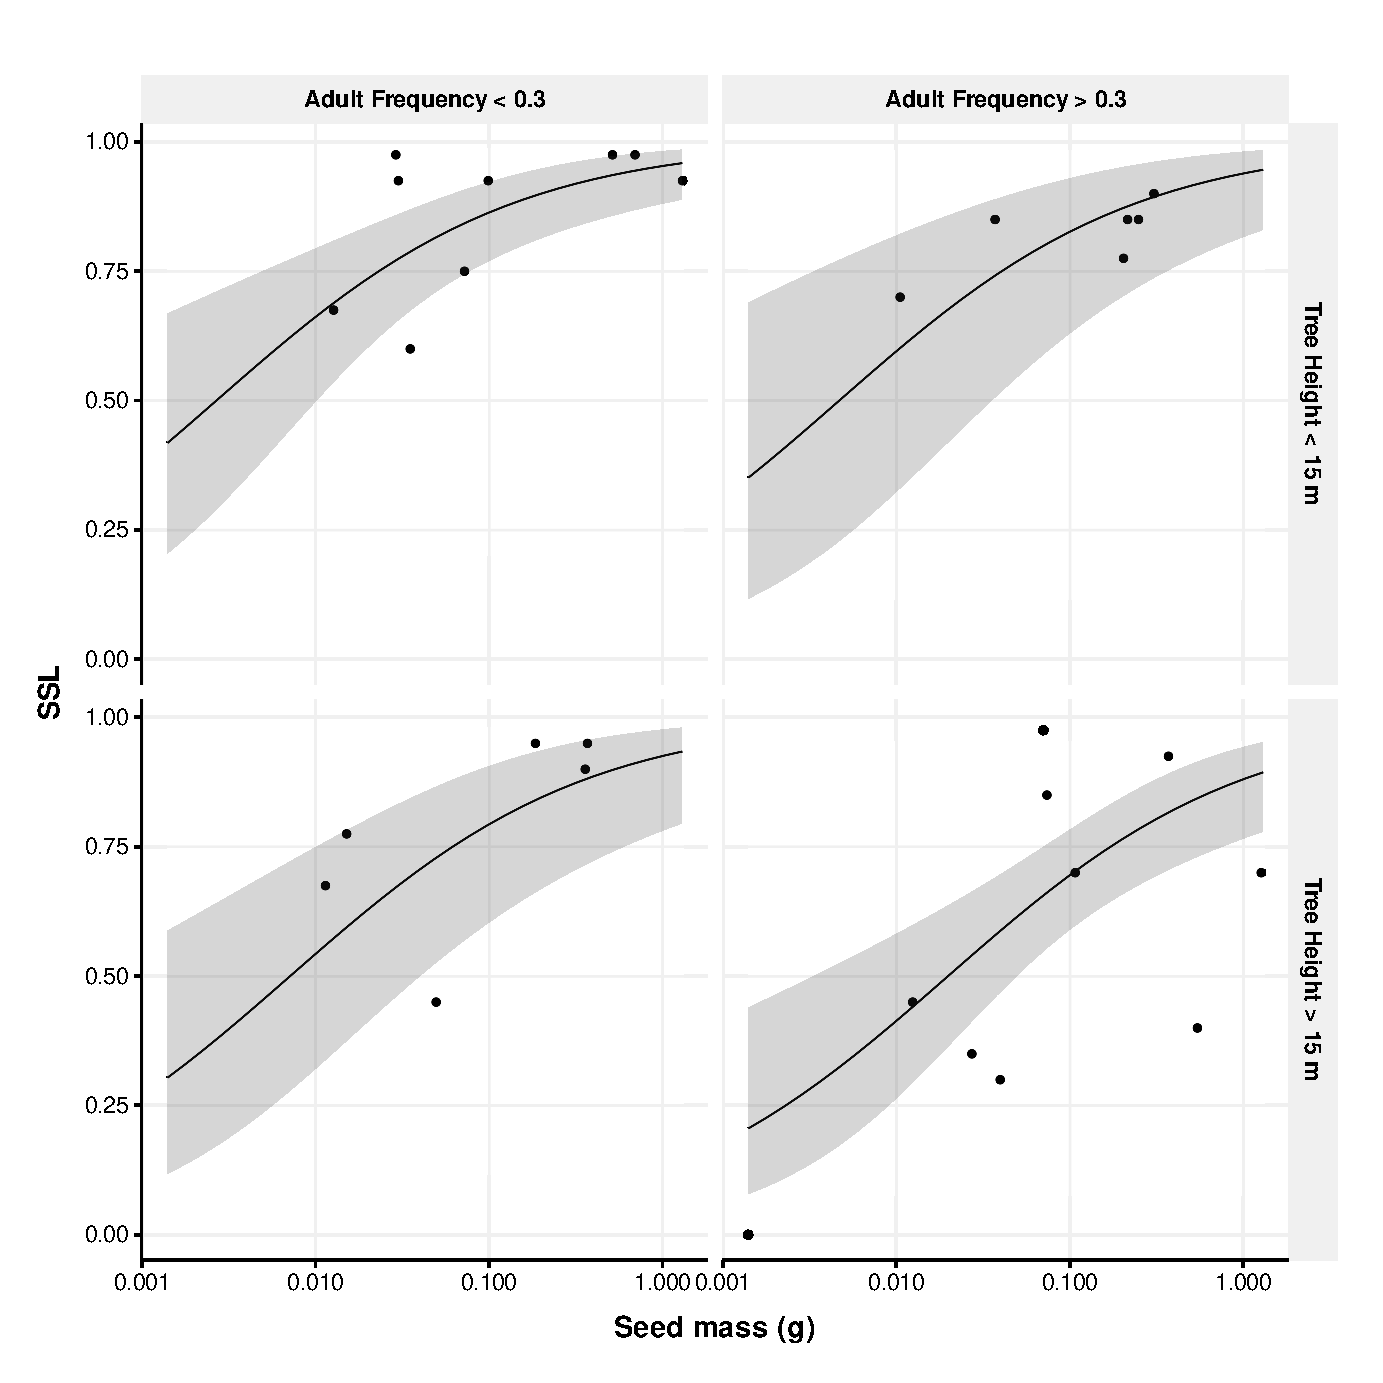
\includegraphics[width=\textwidth]{../figures/SSL_all_pred_prob_glm}
  \caption{Relationship among spatial seed limitation pooled over
    years (SSL), seed mass, tree height, and frequency of adults, as
    predicted by the glm average model (Table~S-3). For species with
    frequency lower than median value (0.3) the relationship is showed
    in graphs in the left column, and for those with greater
    frequency, in the right column. For species with tree height lower
    than median value (15 m) the relationship is showed in upper
    graphs, and for those with greater height in bottom
    graphs. Regression lines are predicted values by the average model
    using the midpoint of the height and frequency class in each
    panel. Gray shadows are 95\% prediction interval of the average
    model. Points are observed values of SSL (pooled over the 3 years)
    and seed mass for each species. Note the log scale for seed mass.}
  \label{fig:SSL_glm}
\end{figure}

\begin{figure}[h!]
  \centering
  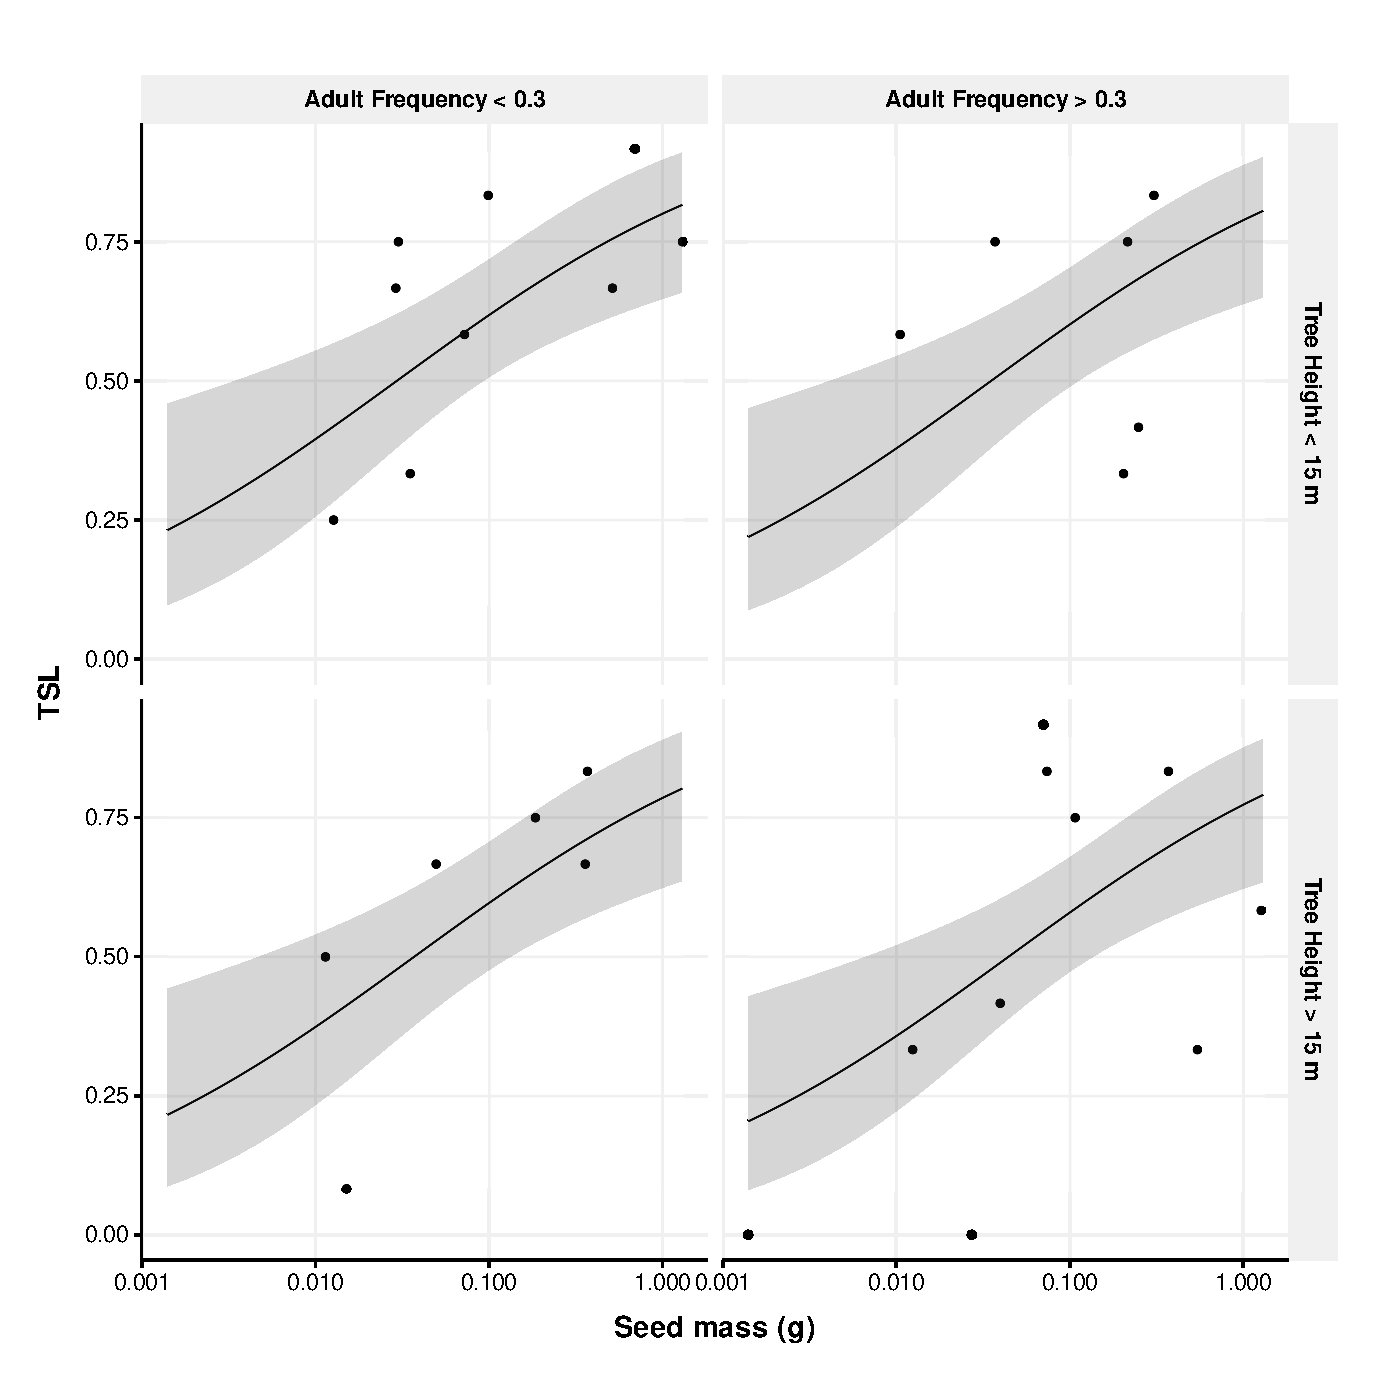
\includegraphics[width=\textwidth]{../figures/TSL_all_pred_prob_glm}
  \caption{Relationship among temporal seed limitation pooled over
    years (TSL), seed mass, tree height, and frequency of adults, as
    predicted by the glm average model (Table~S-4). For
    species with frequency lower than median value (0.3) the
    relationship is showed in graphs in the left column, and for those
    with greater frequency, in the right column. For species with tree
    height lower than median value (15 m) the relationship is showed
    in upper graphs, and for those with greater height in bottom
    graphs. Regression lines are predicted values by the average model
    using the midpoint of the height and frequency class in each
    panel. Gray shadows are 95\% prediction interval of the average
    model. Points are observed values of SSL (pooled over the 3 years)
    and seed mass for each species. Note the log scale for seed mass.}
  \label{fig:TSL_glm}
\end{figure}

\bibliographystyle{plain}
\bibliography{suppl}


\end{document}
